 % !TEX TS-program = pdflatex
% !TEX encoding = UTF-8 Unicode

% This is a simple template for a LaTeX document using the "article" class.
% See "book", "report", "letter" for other types of document.

\documentclass[11pt]{article} % use larger type; default would be 10pt

\usepackage[utf8]{inputenc} % set input encoding (not needed with XeLaTeX)
\usepackage{listings}
%\usepackage{pdflscape}
\usepackage{rotating}
\usepackage{supertabular}
%\usepackage{xtab}

%%% Examples of Article customizations
% These packages are optional, depending whether you want the features they provide.
% See the LaTeX Companion or other references for full information.

%%% PAGE DIMENSIONS
\usepackage{geometry} % to change the page dimensions
\geometry{a4paper} % or letterpaper (US) or a5paper or....
% \geometry{margins=2in} % for example, change the margins to 2 inches all round
% \geometry{landscape} % set up the page for landscape
%   read geometry.pdf for detailed page layout information

\usepackage{graphicx} % support the \includegraphics command and options
\usepackage{subfigure}

% \usepackage[parfill]{parskip} % Activate to begin paragraphs with an empty line rather than an indent

%%% PACKAGES
\usepackage{booktabs} % for much better looking tables
\usepackage{array} % for better arrays (eg matrices) in maths
\usepackage{paralist} % very flexible & customizable lists (eg. enumerate/itemize, etc.)
\usepackage{verbatim} % adds environment for commenting out blocks of text & for better verbatim
\usepackage{subfig} % make it possible to include more than one captioned figure/table in a single float
\usepackage{url} % make it possible to include more than one captioned figure/table in a single float
% These packages are all incorporated in the memoir class to one degree or another...
\usepackage{appendix}

%%% HEADERS & FOOTERS
\usepackage{fancyhdr} % This should be set AFTER setting up the page geometry
\pagestyle{fancy} % options: empty , plain , fancy
\renewcommand{\headrulewidth}{0pt} % customize the layout...
\lhead{}\chead{}\rhead{}
\lfoot{}\cfoot{\thepage}\rfoot{}

%%% SECTION TITLE APPEARANCE
\usepackage{sectsty}
\allsectionsfont{\sffamily\mdseries\upshape} % (See the fntguide.pdf for font help)
% (This matches ConTeXt defaults)

%%% ToC (table of contents) APPEARANCE
\usepackage[nottoc,notlof,notlot]{tocbibind} % Put the bibliography in the ToC
\usepackage[titles,subfigure]{tocloft} % Alter the style of the Table of Contents
\renewcommand{\cftsecfont}{\rmfamily\mdseries\upshape}
\renewcommand{\cftsecpagefont}{\rmfamily\mdseries\upshape} % No bold!

%%% END Article customizations

%%% The "real" document content comes below...

\title{PROJECT PROPOSAL:\\ Development and Implementation of a Fisheries Data Management System}
\author{JS}
%\date{} % Activate to display a given date or no date (if empty),
         % otherwise the current date is printed 

\begin{document}
\maketitle

\tableofcontents

\section{Introduction}\label{Introduction}
The project’s longer-term development objective is to contribute to the sustainable management of the fisheries exploiting the living resources of the Ocean in general, in accordance with the Code of Conduct for Sustainable Fisheries and the Ecosystem Approach to Fisheries.
The immediate objective is to improve the technological (software/hardware) component of the small-scale fisheries monitoring system. For that purpose, we are going to review the existent fisheries management systems, analysing their strengths and their limitations, and propose a set of solutions, based on the latest technologies on databases and Geographical Information Systems.

%speak about hardware and software.
%speak about free and open source, ownership and engaging the community
%Data challenge: recovering data, integrating data and creating new data
%Data quality control
%Interpolating data (intelligence), sampling based metiers
%loose tie architecture (multiple OS components): statistics on R, GIS analysis on Quantum, etc
%Distributed model with embedded devices (mobile phone technology) -  hardware
%Algorithms: fuzzy approach, AI, GIS, 
%technologies: data visualization tools, remote sensing, environmental modelling, Internet, Geo-statistics
%Agile approach: small team, interaction, release often. forums, git, Wiki, meetings, etc
%Deal with different levels of data completeness

%\section{Background and Justification}\label{background}
\section{Background}\label{background}
According to~\cite{fao1}, "decision making for fisheries policy-making, planning and management relies largely on processed information, not raw data". Often the datasets are so large, that the only way to deal with them is through a Database Management System (DBMS). The DBMS in this context may have many functions, but the most relevant ones are: to store the data and ensure its validity and compatibility; it should also be capable of processing it and outputting it, in different ways.

When designing a complete system, many components should be take into account; namely, the User Interface (UI), the data entry, the data processing, the reporting and the Geographic Information Systems (GIS) functionalities (that can be involved in many of the previous steps); the documentation is also something to consider, as it ensures the usability of the system, and some of the reviewed systems also tackle the component of knowledge transfer, through tutorials and workshops. It was not found any system that implemented all of these components, but they seem to focus on some of them instead (for instance,  data processing). As long as the system focus on interoperability, by using open standards and free and open source software (FOSS), this is not a problem since we can combine different systems for our purposes, and avoid in this way, the redundancy on development.

In terms of architecture, there are many options available for building such system; ranging from using complete commercial solutions, by tying together different components, to creating a tailor-made application; all of them have different advantages and inconvenients. In this review, we tried to focus mostly on systems that are already in use, rather than in proposals or assessments of "how" systems should be. This is because to be put in place, fisheries management systems may face many obstacles, such as: burocracy, costs, etc; their ability to cope with them is also part of their success. 

\subsection{General Context}\label{context}
In this section we describe the results of reviewing 25 fisheries management systems. The criteria for selecting the systems that integrate this review, was their visibility; either because they were referred by some colleague, or because they appeared in the internet - as a result of search queries, or within the site of some well-known institution/organisation.

These were some key aspects that were taken into account, when reviewing the systems:
\begin{itemize}
\item security
\item engaging and involvement of stakeholders
\item validation    
\item ability to export information  
\item modular architecture and scalability   
\item licensing     
\item ability to work with incomplete data     
\item status (completed, draft, etc)     
\end{itemize}    
    
Whenever possible the software was tested, but in some cases, where this option was not available, the review is based on user manuals/articles or webpages. Finally it is important to note that often, the systems do not present any information about the type of license, even if sometimes they are distributed at no charge. 

The results of this review, are summarized in a table, on a SQLite database~\cite{bd}. In the next few paragraphs, we are going to analyse the content of this table, reviewing specific characteristics of these systems.

Most of the systems analysed include some sort of database system, to store and manage information (see Figure~\ref{analysis1}a). The DBMS found are very diverse, ranging from free systems such as MYSQL, to expensive proprietary solutions such as Oracle or MS SQL Server. Nevertheless, the majority of the systems use MS Access DB, which although commercial, is low-cost solution (and there are even some free versions). 

\begin{figure}[ht]
\centering
\subfigure[Software use of database;]{
   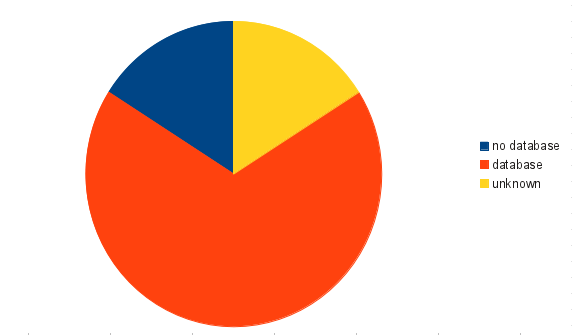
\includegraphics[width=0.8\textwidth] {Chart_database.png}
 }
 \subfigure[Software use of GIS;]{
   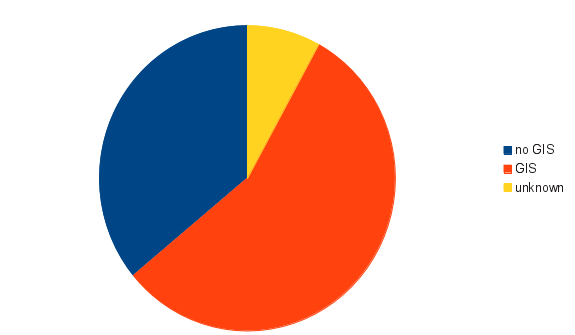
\includegraphics[width=0.8\textwidth] {Chart_gis.png}
 }
\caption[Aggregated analysis of the use of specific software components in the reviewed fisheries management systems;]
{Aggregated analysis of the use of specific software components in the reviewed fisheries management systems;}
\label{analysis1}
\end{figure}

The same conclusion can be drawn about GIS (see Figure~\ref{analysis1}b). The majority of systems uses a GIS component, or has a direct connection with GIS. However, the number of systems without GIS is close to the number of systems with GIS. 

\begin{figure}[ht]
\centering
\subfigure[Need of internet connection, in order to run the software;]{
   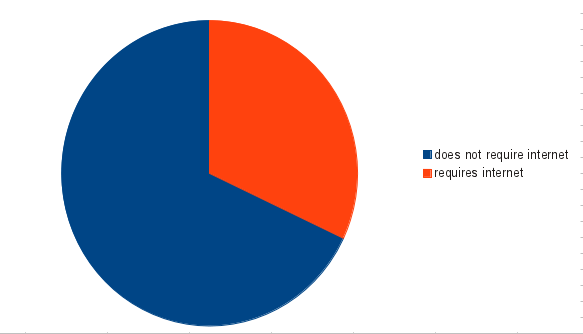
\includegraphics[width=0.8\textwidth] {Chart_internet.png}
 }
 \subfigure[Need for expert knoweledge, in order to use the software]{
   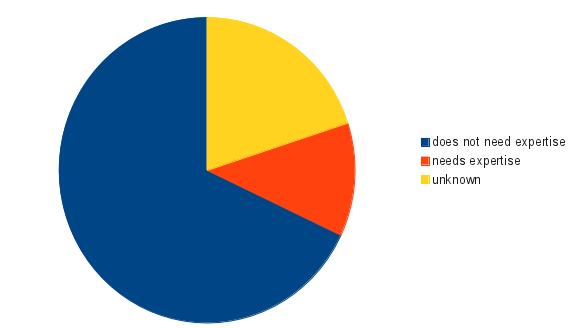
\includegraphics[width=0.8\textwidth] {Chart_expert.png}
 }
\caption[Aggregated analysis of specific characteristics the reviewed fisheries management systems;]
{Aggregated analysis of specific characteristics the reviewed fisheries management systems;}
\label{analysis2}
\end{figure}

As we can see in see figure~\ref{analysis2}a, the vast majority of the reviewed systems does not require an internet connection, in order to work. Also because some of the systems, are low in technology and make little (or no) use of the computer. However, it has to be said, that in modern systems there is an increase use of the server-client architecture, where they centralize the information (database, maps), and serve it through "thin" clients (normally web browsers). The use of web-mapping services such as WMS, triggered a "boom" in the adoption of this kind of model. It is important to note, that although the big advantage of this model is its distributed use, it may also possible to setup it locally on a LAN, or even in a single computer,

Most of the reviewed systems, whether they use software or not, do not present any information about the type of license in place (if any). This can be a consequence of the fact that most of the systems are not distributed, since they are nowhere available for download.

Moreover, most systems do not require a high knoweledge of GIS, databases, statistics, etc, in order to be used (see figure~\ref{analysis2}b). This is either because: costum made solutions were implemented ("tailor-made" software), or widely-known software is used (like for instance MS Access). However, in some cases, specific tools are used that require a bit more literacy (for instance R); in this cases, there is a trade-off since there is something to gain in terms of potentialities of the software allowing to perform more complex tasks, but it is also narrowed the number of possible adopters. 

  \begin{figure}[!ht]%[htbp]
    \begin{center} 
	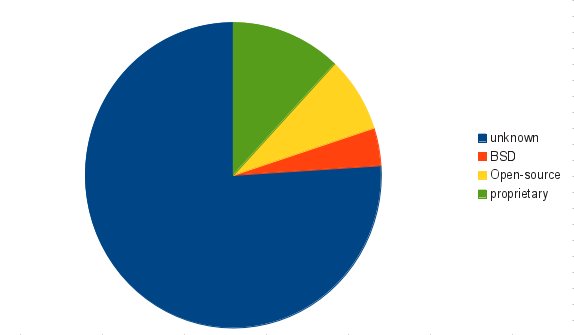
\includegraphics[width=\textwidth ]{Chart_license.png}
      \caption[Software licenses;] {Software licenses;}
      \label{licensing} % so that one can \ref it elsewhere	
    \end{center} 
  \end{figure}

As we can see in figure~\ref{licensing}, most of the reviewed systems, whether they use software or not, do not present any information about the type of license in place (if any). This may be a consequence of the fact that they are not widely distributed (?).

From the systems that especify licenses, there is the same amount of proprietary and open-source type licenses, which clearly indicates the existence of the two segments. Looking at the timeline, there has been an increased adoption of "free and open-source-type" licences, and the expression of interest in adopting these licenses in systems that still rely on proprietary components. This is a very positive trend with great social impacts, specially regarding the adoption of these systems in developing countries.

%\clearpage
The table bellow presents the 25 reviewed systems.

\tablefirsthead{%
\hline
\multicolumn{1}{|c|}{\textbf{Name}} & \multicolumn{1}{c|}{\textbf{Institution}} & \multicolumn{1}{c|}{\textbf{Description}} & \multicolumn{1}{c|}{\textbf{Technical Specifications}} \\ \hline
}
\tablehead{%
\hline
\multicolumn{4}{|l|}{\small\sl continued from previous page}\\
\hline
\hline
\multicolumn{1}{|c|}{\textbf{Name}} & \multicolumn{1}{c|}{\textbf{Institution}} & \multicolumn{1}{c|}{\textbf{Description}} & \multicolumn{1}{c|}{\textbf{Technical Specifications}} \\ \hline
}
\tabletail{%
\hline
\multicolumn{4}{|r|}{\small\sl continued on next page}\\
\hline}
\tablelasttail{\hline}
\bottomcaption{Table-resume of the reviewed Fisheries Management Systems}

\begin{center}
\begin{supertabular}{ | p{0.2\textwidth} | p{0.2\textwidth} | p{0.2\textwidth} | p{0.2\textwidth} |}
Fishframe & ICES & Web- based data warehouse application. It is a plattform for data compilation and tabulating, that allows: upload of information, data quality control, data integration and raising. & Modularized software architecture; server client architecture; browser independent; well specified format; \\ \hline
InterCatch & ICES & Web-based system for handling fish stock assessment data, focusing on documenting characteristics of the catches.  & Client-server architecture (runs on a browser); it uses ASP and SQL Server; \\ \hline
ICES Spatial Facility & ICES & Free interface for searching, viewing and dowloading spatial data. & WMS service (Geoserver) and client (OpenLayers); it was developed in PHP, with an SQL Server database and makes use of the Geonetwork; \\ \hline
ICES EcoSystem Data & ICES & Spatial database; it uses the standards adopted by the user community for the dissemination, visualization and sharing of ICES raw spatial data. & WFS server and client(Geoserver, OpenLayers). MS SQL Server database. \\ \hline
FMS & Schooner Solutions & Software that allows fishermen to track and manage information on daily trap fishing activities; at the same time, it produces reports of catch and effort for the DO. & Stand-alone software that runs on Windows (98 to XP). \\ \hline
The Canadian Albacore Tuna Catch And Effort Relational Database & Oceanic Fisheries Program (SPC) & System that provides annual catch estimates for the Canadian albacore troll fishery based on sales slips, logbooks, and hail Information. & MS Access \\ \hline
TUFMAN & Oceanic Fisheries Program (SPC) & Database fishery management tool. It provides solutions for: data entry, data management, data quality control, administration, and reporting. & Server-client architecture; server in SQL Server and client in MS access (supports the free versions); the mapping is provided through a loose couple with Mapinfo; \\ \hline
Catch and Effort Query System (CES) & Oceanic Fisheries Program (SPC) & Menu-driven system, which allows member countries to extract summaries of operational logsheet data, aggregate public-domain catch and effort data, and annual catch estimates. & It uses Mapinfo for mapping. \\ \hline
Fishery Analyst Online version & MappaMondoGIS & Web-based application, to query fishery data, analyze and visualize temporal and spatial patterns of fishery dynamics. & It uses the Google and ArcGIS JavaScript APIs and the Dojo framework. \\ \hline
Fishery Analyst for ArcGIS 9.x and 10 & MappaMondoGIS & Software for the quantitative estimation and visualization of catch and effort and their variation in space and time, analysis of fishing vessel utilization, data quality control, and deriving information on the location of important economic and threatened species. & Developed in VBA (arcobjects), inside ESRI ArcGIS. The data is stored in DBF files. \\ \hline
FiRST & Collaborative effort across eight South and Southeast (World Fish Center) Asian Countries. & Data management system for scientific trawl survey data. It includes data summary and reporting functionality; outputs: catch, CPUE and biomass estimates. It includes visualization tools, an analytical routine to estimate biomass, and data import/export modules.  & Server-client architecture. Server in MS access/ SQL Server (Windows); client in a browser. \\ \hline
PESCART & Instituto Nacional de Investigação Pesqueira (IIP) & Database system for storing data from artisanal fisheries and efectuate some calculus and reports (catch, effort, CPUE). It includes an interface for data acquisition, analysis and reporting. & Developed in Microsoft Access 97 (Windows 98); the system is split in two databases: one containins the data and the other one the app (UI+processing); it uses some MS specific ActiveX (Microsoft FlexGrid Control 5.0) and Libraries (.e.g DAO) \\ \hline
Geocrust & University of Algarve (UALG) & System that uses Satellite data (VMS) to map effort and landings;  & Modular stand-alone application with embebed GIS. It was developed using: Visual Basic 6.0., ADODB and MapObjects 2.0 Pro. It uses a MS Access Database (2000). \\ \hline
Geocrust 2.0 (Geopescas) & University of Algarve (UALG) & Improvement of the Geocrust application, as a consequence of extending the methodology to the ground fish trawl flee, a larger period, and a larger geographical area. & The db was migrated to MySQL running on a Linux server (higher security). It were introduced Artifical Intelligence methods (automatic classification methods) for trawl detection, in addition to the manual procedures. \\ \hline
Geopescas Website & University of Algarve (UALG) & Website to disseminate geo-referenced information on fishing effort, landings, catches and catch rates, through fisheries researchers, fishery administration and fishing industry. It shows some of the maps generated by the Geocrust software and it offers dynamic mapping, using Geotools. & It uses the Geoserver mapping component, costumised through JAVA programming. \\ \hline
COST & Project financed by the European Commission under the call FISH/2006/15 – lot 2 & Open Source Tool for raising and estimating properties of statistical estimates derived from the Data Collection Regulation. & set of R libraries, with the following functionalities: import and handle fisheries data, explore the data , estimate the parameters and related precision and do simulation. It relies on data in a well specified forma.t \\ \hline
Catch Assessment Survey and Statistical frame survey of the artisanal fisheries of Kontagora Reservoir & ? & Catch Assessment Survey and Statistical frame survey, that aims to sustain the formulating of management plan and policies for the Kontagora reservoir. & Count and weighting of the fish. \\ \hline
Artisanal Fisheries Data Collection And Management In Tanzania & UNU Fisheries Training Program Fisheries Division - Statistical Unit  & Simple sampling procedure, community based data collection model and specifying of types of data to be collected. This system also includes analysis methods and a "tax motivation" strategy. & MS excel, MS Access Database. \\ \hline
IFMP & Lake Victoria Fisheries Organisation (LVFO)  & Catch Assessment Surveys, two-stage stratified sampling design and estimation of CAS-based Indicators. & data forms (paper), MS Excel. \\ \hline
Barahona Data Collection System & Barahona Data Col PROPESCAR-SUR project & National Data Collection System & it relies on paper records and the calculations are done" by hand". \\ \hline
Samaná Fisheries Development Project (CEDEP) & Japan? & Logbook recording system, for a small number of vessels. & ? \\ \hline
FISBOAT & IFREMER & Fisheries Independent Survey-Based Operational Assessment Tools. The tools tackle the major issue of unreliable fish stock assessment, through the use of new methods based exclusively on research vessel survey data. & R, FLR simulation framework (R based) \\ \hline
Probability-based survey techniques in Mozambique & Instituto Nacional de Investigação Pesqueira (IIP) & Probability-based survey techniques for monitoring catch and effort in the coastal small-scale fisheries. & onsite survey, database (?) \\ \hline
Programme for refining estimates of local fishery production in Western Samoa & Peace Corps Marine Biologist Fisheries Division, Western Samoa & A programme for refining estimates of local fishery production, that consists in data collection(interviews) and data analysis; & It uses written down interviews to collect data and a hand-held programmable calculator for analysis; as a database, it is used DBASE III. \\ \hline
Electronic Fish Catch Logbook Project (EFCL) & Northwest Fisheries Centre (NWFSC) & Ship-based software and shore-based web application to collect and report logbook, catch "(fish tickets"), biological sample and observer data. There is also a report system, a central database and web based app to upload data. & Client server architecture, Oracle database, Arcinfo GIS; \\ \hline
\end{supertabular}
\end{center}
%\label{}
%\end{table}

In the following table, the reviewed systems are organized according to their technical characteristics:
\begin{itemize}
\item {\it internet}: indicates if the software needs an internet connection to work (binary value);
\item {\it GIS}: indicates if the software uses GIS (binary value);
\item {\it database}: indicate if the software uses a database (binary value);
\item {\it license}: indicates the type of license;
\item {\it portability}: comments about the cross-platform ability;
\item {\it expertise}: indicates if there is the need of expert knoweledge to run the system (binary value);
\item {\it released}: indicates if the system is released and already in use; 
\end{itemize}

\tablefirsthead{%
\hline
\multicolumn{1}{|c|}{\textbf{Name}} & \multicolumn{1}{c|}{\textbf{internet}} & \multicolumn{1}{c|}{\textbf{GIS}} & \multicolumn{1}{c|}{\textbf{license}} & \multicolumn{1}{c|}{\textbf{database}} & \multicolumn{1}{c|}{\textbf{portability}} & \multicolumn{1}{c|}{\textbf{expertise}} & \multicolumn{1}{c|}{\textbf{released}} \\ \hline
}
\tablehead{%
\hline
\multicolumn{8}{|l|}{\small\sl continued from previous page}\\
\hline
\hline
\multicolumn{1}{|c|}{\textbf{Name}} & \multicolumn{1}{c|}{\textbf{internet}} & \multicolumn{1}{c|}{\textbf{GIS}} & \multicolumn{1}{c|}{\textbf{license}} & \multicolumn{1}{c|}{\textbf{database}} & \multicolumn{1}{c|}{\textbf{portability}} & \multicolumn{1}{c|}{\textbf{expertise}} & \multicolumn{1}{c|}{\textbf{released}} \\ \hline
}
\tabletail{%
\hline
\multicolumn{8}{|r|}{\small\sl continued on next page}\\
\hline}
\tablelasttail{\hline}
\bottomcaption{Reviewed Fisheries Management Systems, according to their characteristics}

\begin{center}
\begin{supertabular}{ | p{0.1\textwidth} | p{0.05\textwidth} | p{0.05\textwidth} | p{0.05\textwidth} | p{0.05\textwidth} | p{0.2\textwidth} | p{0.05\textwidth} | p{0.05\textwidth} |}
Fishframe & 1 & 1 & BSD & 1 & Since the clients are browser based, they are cross platform; the server has to run on Windows, since it uses Microsoft specific active technologies (ASP) & 0 & yes \\ \hline
InterCatch & 1 & \multicolumn{1}{l|}{?} & ? & 1 & Since the clients are browser based, they are cross platform; the server has to run on Windows, since it uses Microsoft specific active technologies (ASP) & \multicolumn{1}{l|}{?} & ? \\ \hline
ICES Spatial Facility & 1 & 1 & ? & 1 & Server and client are cross-platform. & 0 & yes \\ \hline
ICES EcoSystem Data & 1 & 1 & ? & 1 & Server and client are cross-platform. Database is Windows specific. & 0 & yes \\ \hline
FMS & 0 & \multicolumn{1}{l|}{?} & proprietary & \multicolumn{1}{l|}{?} & Windows only (98 to XP) & \multicolumn{1}{l|}{?} & under final modifications \\ \hline
The Canadian Albacore Tuna Catch And Effort Relational Database & 0 & 1 & ? & 1 & Windows only & 0 & yes \\ \hline
TUFMAN & 0 & 1 & ? & 1 & Windows only & \multicolumn{1}{l|}{?} & yes \\ \hline
Catch and Effort Query System (CES) & 0 & 1 & ? & 1 & Windows only & 0 & yes \\ \hline
Fishery Analyst Online version & 1 & 1 & proprietary & \multicolumn{1}{l|}{?} & The client is free and cross plattform (runs on a browser) & 0 & yes \\ \hline
Fishery Analyst for ArcGIS 9.x and 10 & 0 & 1 & proprietary & 1 & Windows only & 1 & yes \\ \hline
FiRST & 1 & 1 & ? & 1 & Since the client runs on a browser, it is platform independent. Server runs on Windows. & 0 & yes \\ \hline
PESCART & 0 & 0 & ? & 1 & Windows only & 0 & yes \\ \hline
Geocrust & 0 & 1 & ? & 1 & Windows only & 0 & yes \\ \hline
Geocrust 2.0 (Geopescas) & 0 & 1 & ? & 1 & The application runs on Windows, but the database can now run on Windows or Linux. & 0 & yes \\ \hline
Geopescas Website & 1 & 1 & ? & 1 & ? & 0 & demo version only \\ \hline
COST & 0 & 1 & Open-Source & 1 & since it relies in R, it is cross-platform. & 1 & yes \\ \hline
Catch Assessment Survey and Statistical frame survey of the artisanal fisheries of Kontagora Reservoir & 0 & 0 & ? & \multicolumn{1}{l|}{?} & ? & 0 & yes \\ \hline
Artisanal Fisheries Data Collection And Management In Tanzania & 0 & 0 & ? & 1 & Windows only & 0 & yes \\ \hline
IFMP & 0 & 0 & ? & 0 & Windows only & 0 & yes \\ \hline
Barahona Data Collection System & 0 & 0 & ? & 0 & n/a & 0 & yes \\ \hline
Samaná Fisheries Development Project (CEDEP) & 0 & 0 & ? & 0 & ? & \multicolumn{1}{l|}{?} & yes \\ \hline
FISBOAT & 0 & 0 & Open-source & 0 & multi-platform & 1 & yes \\ \hline
Probability-based survey techniques in Mozambique & 0 & 0 & ? & \multicolumn{1}{l|}{?} & ? & \multicolumn{1}{l|}{?} & yes \\ \hline
Programme for refining estimates of local fishery production in Western Samoa & 0 & 0 & ? & 1 & Windows only (DOS) & 0 & yes \\ \hline
Electronic Fish Catch Logbook Project (EFCL) & 1 & 1 & ? & 1 & Some components run on a browser, so they may be cross-plattform, but the database and GIS are Windows only. & 0 &  \\ \hline
\end{supertabular}
\end{center}

The next table, goes a bit more in depth, and it analyses some of the advantages and disadvantages of each system. 

\tablefirsthead{%
\hline
\multicolumn{1}{|c|}{\textbf{Name}} & \multicolumn{1}{c|}{\textbf{Advantages}} & \multicolumn{1}{c|}{\textbf{Disadvantages}} \\ \hline
}
\tablehead{%
\hline
\multicolumn{3}{|l|}{\small\sl continued from previous page}\\
\hline
\hline
\multicolumn{1}{|c|}{\textbf{Name}} & \multicolumn{1}{c|}{\textbf{Advantages}} & \multicolumn{1}{c|}{\textbf{Disadvantages}} \\ \hline
}
\tabletail{%
\hline
\multicolumn{3}{|r|}{\small\sl continued on next page}\\
\hline}
\tablelasttail{\hline}
\bottomcaption{Advantages and disadvantages of each system}

\begin{center}
\begin{supertabular}{ | p{0.3\textwidth} | p{0.3\textwidth} | p{0.3\textwidth} |}
Fishframe & - data ownership of the recipients; - deals with incomplete data; - cross plattform); - enforces confidentiality; - involvement and engagement of stakeholders; - bottom-up approach & - some components require Windows XP; - development is Windows based; - for complex tasks the browser solution is not efficient; \\ \hline
InterCatch & ? & It uses proprietary and platform-specific software \\ \hline
ICES Spatial Facility & - cross platform (browser based); - adopts OGC standards; - friendly UI; - uses Free and Open Source Software( FOSS); & There is no component of data acquiring in this system; it is assumed the raw data is validated. \\ \hline
ICES EcoSystem Data & - cross platform (browser based); - adopts OGC standards; - friendly UI; - uses Free and Open Source Software( FOSS); & - some requests may be slow due to the quantity of data; - - it deals only with survey data; \\ \hline
FMS & It does not require a very powerful hardwareto run. & - it runs only on windows; -it has a cost; \\ \hline
The Canadian Albacore Tuna Catch And Effort Relational Database & - it deals with unreported catch; - although it is a post-season analysis tool, in can be used as in-season analysis (based only on trip logs); & - the results may be biased due to the use of logbooks without saleslip data; - other sources of bias are the "public sales" and "take homes" that are not registered anywhere (they "escape" from logbook and sales slips);  \\ \hline
TUFMAN & - the website provides excelent documentation on how-to use the application; - flexible system, able to cater the needs of each country; - it allows to identify gaps in data; & - it uses proprietary components (Mapinfo, Microsoft Office Pro); - it does not feature data acquisition, and therefore it is dependent on the quality of input data; - it does not provide tools to fill the gaps in the data; - it is not found anywhere to download; \\ \hline
Catch and Effort Query System (CES) & - developed reporting facilities, with the use of graphs, tables and maps; & - it uses proprietary components (Mapinfo); - it is not found anywhere to download; \\ \hline
Fishery Analyst Online version & - lightweight and cross-platform application; & -it has a cost; \\ \hline
Fishery Analyst for ArcGIS 9.x and 10 & - it takes advantage of GIS to analyse geodata; - it provides a time series animation; - it provides data quality contro routines; - it uses; transversal information (economical); - confidentiality is addressed; & - it has a cost, although a demo version is provided for free; - it requires ArcGIS 8.3. or 9 with Spatial Analyst (and it needs this specific versions to work); - it requiressome knoweledge of ArcGIS to use; - it requires some detailed georeferenced data to start with (no estimation provided!) \\ \hline
FiRST & - client is cross plattform; - no installation required for the client; - a regional database is “compiled” from the national databases; - outputs can be used for ecological modelling (very usefull for management – devise or revise zonation schemes); & - the database is designed for scientific trawl surveys; - it requires installation of a webserver; - the exporter uses mostly proprietary formats (MS Office, Crystal reports, MS Access); \\ \hline
PESCART & - intuitive UI following the information flow; - it is a very complete system, since it covers: data acquisition, estimation and reporting. & - it targets artisanal fisheries only (the basic unit is fishing unit); - "bulky" setup with a lot of requirements; - the application does not have any access restrictions (no permission system implemented); - the limitations of MS Access "clash" with the design of the app (e.g. number of fields on a table does not allow the selection of a large number of species;) \\ \hline
Geocrust & - it combines positioning and landing data, from different sources (IGP, DGPA, logbooks); - extense use of GIS, not only for display but also for calculations (e.g.: buffers to define start and end of fishing trips); - it is generic enough, to be used with other fleets/geographic areas/species; & - it is based on proprietary technologies; - it relies on accurate positioning data (VMS); - it was not addressed a permission model for the UI (only superuser); \\ \hline
Geocrust 2.0 (Geopescas) & - the procedure of identification of trips was enhanced with AI; - DBMS was migrated to a free, multi-platform software; & - it is still based on proprietary technologies; - the AI procedure needs adequate "training", in order to produce good results; \\ \hline
Geopescas Website & - it provides an interface for querying maps; - it exports georeferenced maps, images and XML, that can be integrated in third-party apps.  & - it depends on technologies Ggeotools) that are heavy on the browser and require the installation of the Java plugin; - it was only released a demo version; \\ \hline
COST & - space dimension is included in the analysis; - uses well known technology; - promotes import and export of data; - open source and cross plattform tool; - interfaces with Fishframe format; & - relies in good quality and well formatted data; - it requires expert knoweledge; \\ \hline
Catch Assessment Survey and Statistical frame survey of the artisanal fisheries of Kontagora Reservoir & - it is a complete system, including data collection (survey) and statistical analysis of the results; - it comprehends both effort and catch; & Although the data is collected spatially, there is no indication that this component is taken in account in the sampling and analysis. \\ \hline
Artisanal Fisheries Data Collection And Management In Tanzania & - relatively inexpensive; - it does not need specialized staff to run and maintain it; - it contemplates the community participation; & There is no reference to GIS in the sampling procedure (although the sampling is on space), or in the estimation process. \\ \hline
IFMP & - it provides estimations of the catch over the years, which allows to detect trends, to detect need for further data and to evaluate management interventions. & - since data collection is through papper sheets, there is no data quality control on introduction; - there is no mention of a solution to store and manage the data over time (DB); - there is no use of GIS, although the PSU are spatial; \\ \hline
Barahona Data Collection System & - the economic variables are well catered; - it gathers relatively accurate catch and effort information based on trip interviews; The effort variables, in particular, seem well thought out and adequate for monitoring CPUE and estimating fishing mortality; - the system was sustained, even after withdrawl of external funding; & - mortality and growth cannot be estimated with current data ; - there is the need for a new approach fro estimating discards; - the current sampling procedure does not follow a statistically rigorous method. - there is no database to store and manage data on a long term; - there is the need of training; - stock assessment is not contemplated in this system; \\ \hline
Samaná Fisheries Development Project (CEDEP) & - data collection is rigorous; & - the logbooks are not formally structured; - the data is not mantained in a database; \\ \hline
FISBOAT & - these tools provide robust and reliable scientific advice to fishery managers and policy-makers, including a management model driven by numerically defined harvesting rules; - it is provided an early-warning mechanism, giving policy-makers more time to respond proactively to evolving challenges. & - the methods are based exclusively on research vessel survey data; - it requires expert knoweledge to be used (statistics and computation); \\ \hline
Probability-based survey techniques in Mozambique & - the probability sampling produces unbiased estimates of catch, effort, and other key parameters; - the precision in such estimates can be quantified; - it is cost-effectiv; - the underlying theory is well developed and documented; & - no mentioning of use of GIS; \\ \hline
Programme for refining estimates of local fishery production in Western Samoa & - cost-effective method of gathering basic information that provides clues to changes in the fishery as a whole; - it requires a small input of resources for the information obtained; & - the data quality of the survey is threatened by the hiring of causal workers, without adequate supervision; the same for data entry in the database; - outdated database techology; - there is the need to collect more data (from the villages) to estimate the catch; - there is the need to design more complete entry datasheets; \\ \hline
Electronic Fish Catch Logbook Project (EFCL) & - innovative effort to automate and standardize logbook data. - it implements permissions through roles; - it supports secure connections (data encryption) - the use of a software to input the raw data, allows a first validation layer that does not exist in traditional systems using papper sheets; - costumisable;  & - it is based in proprietary technologie; - it relies on internet access for data uploads and visualisation; \\ \hline
\end{supertabular}
\end{center}

%Many systems have been developed on the past few years, in order to address the modern challenges of fisheries data management. Some of these systems (like for instance Fishframe~\cite{fishframe}) developed quite a lot some components of the system such as data importing or validation but did not cover other components, such as raw data acquiring which being the first step, is in many cases essential for the overall functioning of the system. There are also many examples of systems (\cite{fishframe},~\cite{intercatch}) which use the web has a primary interface and therefore require a stable Internet connection, with a significant bandwidth; although this is desirable, and progressively more common, it is not always the scenario we encounter in developing countries, and therefore this fact should be taken in account when planning and designing a system that should reach the maximum number of adopters.\\
%Although free and/or open source is increasingly recognized as a valuable development and licensing model and some fisheries management systems had already adopt it (see~\cite{fishframe}), the  fact that they still rely partially or fully in proprietary software, like for instance MS Access (see \cite{intercatch},~\cite{tuna}), prevents them from fully enjoying the advantages of such a model; these advantages include, amongst many other things, the zero development cost that can increase the software ownership by countries with limited budgets (see section~\ref{objectives}).\\
%Unfortunately, FishFrame, Intercatch and the Canadian Albacore Tuna Catch and Effort Relational Database System are still not the rule, and in many places such as Dominican Republic, Western Samoa or Uganda, the technological component and automation of tasks are still in their early stages (see~\cite{victoria},~\cite{dominican},~\cite{samoa}); data collection methods are still limited to sheets of paper and databases are still not implemented to store and manage this data; needless to say GIS as modelling/visualization tools are nearly inexistent, although the "need" of a spatial support for information is clearly shown by hand-drawn maps.\\
In the next section (see~\ref{objectives}) we present a set of fisheries management tools that pretend to fill some of these "gaps" on existent systems, reusing some of its (good) ideas and adding new technologies that are "giving cards" on other fields (like fuzzy mapping, on section~\ref{output}, or artificial intelligence), having in mind the limitations and potentialities of the recipients (developing countries). Some of these ideas also arise during the development of Medfisis-CAS~\cite{medfisis}, an (almost) full and open-source system that reunites data from Logbook and Artisanal Fisheries in the same application/database; some of the concepts developed during this project such as abstractability of entities and configurability of components can be very useful in all stages of Fisheries Management Systems.\\
Figure~\ref{challenges} shows some of the challenges that can be addressed by a set of fisheries management tools. We propose a loose couple architecture, where we maximize the use of existing tools: to cut development time, to benefit from their value and also to involve a community of users that can take advantage of their expertise in specialized tools (like for instance R, or QGIS) to push the system further. The modularization of the system also means that we can distribute tasks, and till a certain extent develop them independently without compromising the rest of the system.\\

%open source
%creation of a community /AGILE model for development
%improvement of the manuals
%success stories in other areas 

  \begin{figure}[!ht]%[htbp]
    \begin{center} 
	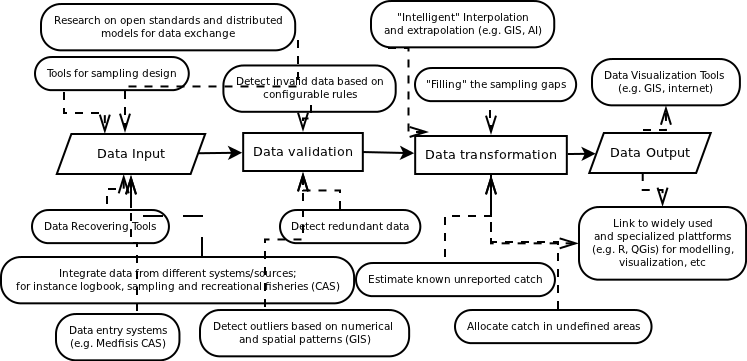
\includegraphics[width=\textwidth ]{challenges_cas.png}
      \caption[Some Interesting Challenges on Fisheries Management Systems;] {Some Interesting Challenges on Fisheries Management Systems;}
      \label{challenges} % so that one can \ref it elsewhere	
    \end{center} 
  \end{figure}


\section{Project Objectives}\label{objectives}
The design of a software system for fisheries management, as described in section~\ref{background} (figure~\ref{challenges}), should contemplate four stages:
\textbf{input, validation, transformation and output}. The main target for each of this stages is the data about fisheries, in its raw or transformed state (catch, efforts), but it can also be other (complementary) types of data (meteorological, oceanographical, socio-economic, etc). In the following subsections we identify a serious of tasks that are \textit{on-demand}, and could result in very useful tools for fisheries scientists and managers. They are not limitative, and in our modular design they can be seen as a first approach rather than a complete description of the system.\\

\subsection{Data Input}\label{input}
The data input component contemplates the collection of information for the system, either by creating this information "from scratch" or by importing it from different supports/formats.

\begin{itemize}
  \item \textbf{Tools for Sampling Design}: Before even introducing information in the system, it is often necessary to collect this information; the design of a an unbiased sampling scheme, that minimizes the costs and maximizes the quality of the results it is an important and often overlooked task; overlooked, because many times the designer is not provided with the necessary tools to make it an easy and efficient process. There are many advantages of using a spatial framework (GIS) on this particular problem, and suggestions can guide the sampler to informed and wise decisions.
  \item \textbf{Research on Open Standards and Distributed Models for Data Exchange:} The problem of exchanging data between different instances of the system is a pertinent and frequent one. JSON~\cite{json} and SQLite~\cite{sqlite} are open and well-known standards that are "light" alternatives to XML. Also, the design and implementation of a server-client model, where we leave the "heavy processing load" to the server and create "light" data acquiring clients (for instance running on mobile phones and Ipads) can simplify the task of data integration, as we only update restricted parts of the system.
  \item \textbf{Data Recovering Tools:} There is a large quantity of historical data that is lost in terms of its value, just because it is not in an usable format. Data series take many years to assemble, and not only it costs a lot of money to generate new data, but it is not actually possible to recreate past information, so when this information is lost it is lost forever. It could be a very rewarding task to at least try to compile this information, that may not be usable for different reasons; hard disks that have bad sectors, obscure data formats whose specification was lost, data in non digital support and nearly illegible: these are all problems eligible for "data archaeology", that can make use of advanced software techniques such as: writing recognition, deyncription algorithms and hard-disk recover tools.
  \item \textbf{Integrate data from different systems/sources:} The integration of different types of information provides a rich basis for the analysis and transformation of information; this includes having data from different sources such as oceanographical, meteorological, sociological, etc; apart from implementing a system that is able to import different formats (satellite images, excel spreadsheets, vector maps, etc) it is also relevant to design a system that can deal with the nature of this variability - for instance recreational fisheries data, logbooks and sales slips can be integrated with a unified and generic design and provide a richer basis for fisheries statistical analysis (see~\cite{medfisis}).
  \item \textbf{Data Entry User Interfaces:} Database clients are a \textit{milestone} in fisheries applications and common examples of this are digital logbooks and fleet register software's (see~\cite{medfisis}). They reproduce the behavior of paper sheets for data collection, with all the advantages of data checking, and "feed" directly the database; if they are well designed and the data operators are trained, are also quicker and more friendly to use than the replaced papper sheets. There is still a room for improvement on this UIs, for instance enabling multiple choices or configurable validation rules~\footnote{As an example, some of this features were already implemented in CAS Medfisis~\cite{medfisis}}.
\end{itemize}

  \begin{figure}[!ht]%[htbp]
    \begin{center} 
	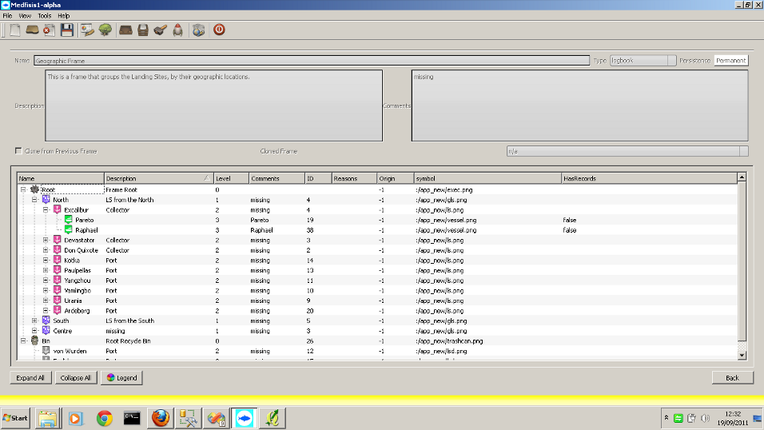
\includegraphics[width=\textwidth ]{geographic_frame}
      \caption[This \textit{tree-like} widget is a tool developed in Medfisis~\ref{medfisis} to assist in the design of a sampling frame; the user can drag and drop elements from one group to another, which can be an interesting feature for designing sampling schemes;] {This \textit{tree-like} widget is a tool developed in Medfisis~\cite{medfisis} to assist in the design of a sampling frame; the user can drag and drop elements from one group to another, which can be an interesting feature for designing sampling schemes;}
      %\label{challenges} % so that one can \ref it elsewhere	
    \end{center} 
  \end{figure}


  \begin{figure}[!ht]%[htbp]
    \begin{center} 
	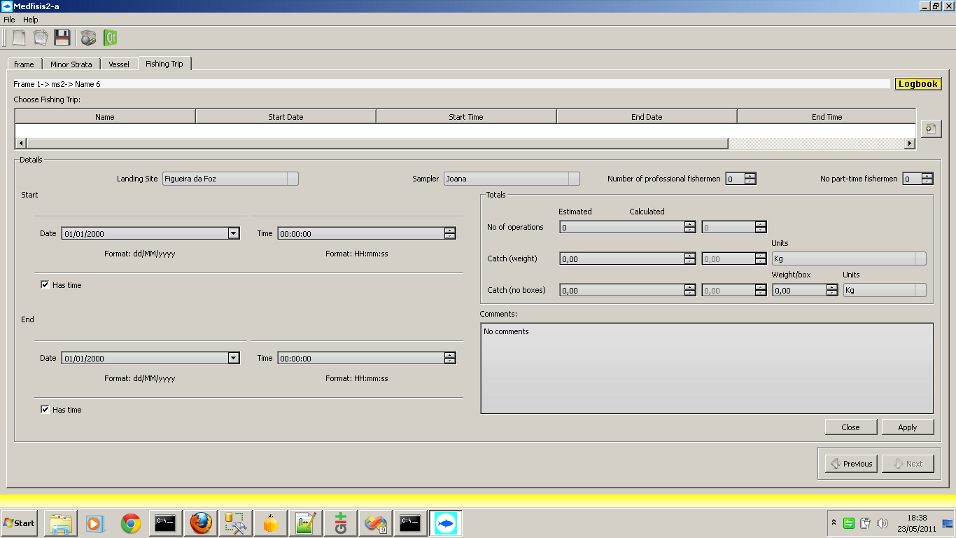
\includegraphics[width=\textwidth ]{fishing_trip_small}
      \caption[Screenshot of a data entry form for fishing tip data, on CAS Medfisis~\cite{medfisis}; on this system, forms were designed to accommodate at the same time logbook and artisanal fisheries data;] {Screenshot of a data entry form for fishing tip data, on CAS Medfisis~\cite{medfisis}; on this system, forms were designed to accommodate at the same time logbook and artisanal fisheries data;}
      %\label{challenges} % so that one can \ref it elsewhere	
    \end{center} 
  \end{figure}

\subsection{Data Validation}\label{validation}
Since the data entering the system may arrive from sources other than its data generator interfaces\footnote{The data entry interfaces should have already their own validation routines removing, at least partially, the need for this step.}, it is important to control the quality and validity of information we are inputing; this step is fundamental for all the following ones, since "bad quality" data will compromise the entire system ("garbage in, garbage out").\\
The Fishframe application~\cite{fishframe}, developed by the Danish Institute for Fisheries Research, presents an interesting and complete multi-step validation layer; on a first stage it is performed a basic check, looking at the structure of the data, ranges of values and duplicate values; on a second stage, a more complex check searches for the correctness of the dependency between fields; finally, the last check (which is not compulsory) performs a global analysis, looking at the general patterns in order to identify outliers. Apart from this, it also allows some customizable checks to be introduced by the user, that can be performed automatically. This flexibility and completeness of the validity step, inspired us to identify the following tasks in the data validation component of this system:

\begin{itemize}
  \item \textbf{Detection of redundant data}: The detection (and consequent removal) of duplicate records is an important task, in order to have a "clean" database. It is not complicate to identify automatically records that are \textbf{exactly} identical, but the problems arise when we have for instance spelling mistakes, and records that are \textit{almost} the same, but not exactly the same. As this situations are dubious, and may correspond or not to duplicate data, they require user supervision to confirm it; however, there is no reason why they can not be identified and presented to the operator has "possible duplicates"; for this task, it is very useful to use data mining techniques such as a fuzzy approach to language~\cite{fuzzy}.

  \item \textbf{Detection of invalid data based on configurable rules}: Generic rules can be applied to check for the correctness of the data types, correctness of keys, etc, directly based on the database schema. However, some rules such as the format of strings, ranges of values, may change from system to system  (for instance according to the geographic location) and the option to create them should be left to the user. To avoid "hard-coding" of rules, which would require a programmer's intervention and consequently difficult the process of exploratory analysis, we propose an interface for user configurable rules. This interface can be similar to a query builder such as the one represented in~\ref{builder}, which may be familiar to some users.

  \item \textbf{Detection of Outliers}: Outliers might arise due to careless data acquiring, instrument malfunction, wrong data processing routines, or any other reasons~\cite{outliers}; generic methods based on tabular data (for instance using a principal component analysis) can be used to perform this task, but there is also room for other techniques such as data mining, or GIS; for data with a spatial distribution (which is often the case in fisheries) GIS can provide a very valuable tool for capturing the general spatial pattern and consequently the values that fall outside this pattern (outliers)(see figure~\ref{dem}).
  After detecting and removing outliers values, we are left with the problem of imputation of "missing values" to replace the removed information (see section~\ref{transformation})

\end{itemize}

  \begin{figure}[!ht]%[htbp]
    \begin{center} 
	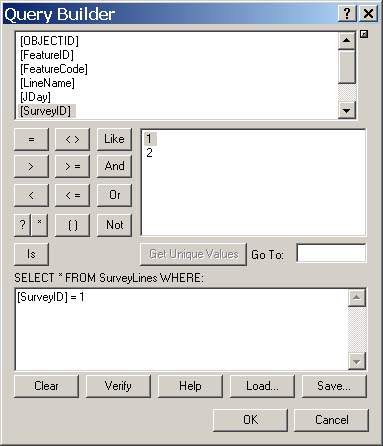
\includegraphics[width=0.5\textwidth ]{builder.jpg}
      \caption[Query builder from ArcGIS;]
{Query builder from ArcGIS; source:~\url{http://woodshole.er.usgs.gov/pubs/of2006-1381/html/fig19.html};}
      \label{builder} % so that one can \ref it elsewhere	
    \end{center} 
  \end{figure}

  \begin{figure}[!ht]%[htbp]
    \begin{center} 
	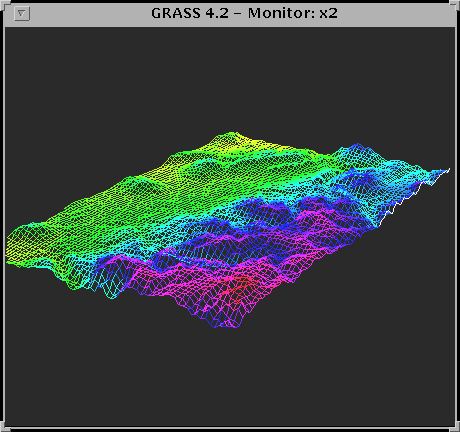
\includegraphics[width=0.8\textwidth ]{dem.png}
      \caption[A Digital Elevation Model (DEM) like the one above, can be used to generate a surface of values in order to detect outliers;]
{A Digital Elevation Model (DEM) like the one above, can be used to generate a surface of values in order to detect outliers; source:~\url{http://www.grass-kr.org/research/demo1/index.html};}
      \label{dem} % so that one can \ref it elsewhere	
    \end{center} 
  \end{figure}


\subsection{Data Transformation}\label{transformation}
Data transformation consists in using the information in the system and apply transformations to it, in order to generate new information. These transformations may be used to estimate values extending the scope of the dataset, or to generate indicators that characterize the dataset, like for instance the CPUE, or both. In this system we suggest facilitating the export of data and leave (some) more complex data analysis to specialized software such as R (figure~\ref{lengths}) or QGis(figure~\ref{layers}).

  \begin{figure}[!ht]%[htbp]
    \begin{center} 
	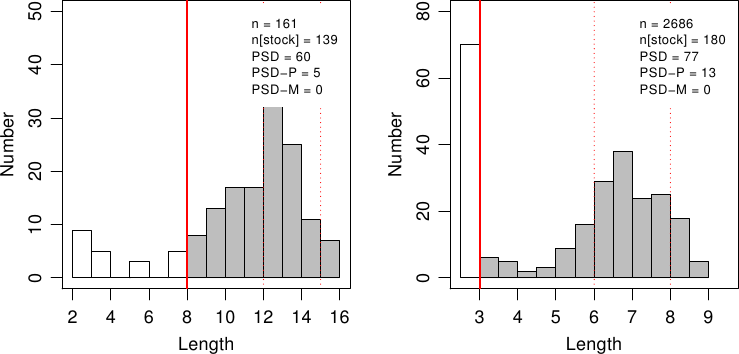
\includegraphics[width=\textwidth]{lengths}
      \caption[This analysis of the size structure was created using the R package;]
{This analysis of the size structure was created using the R package; source:~\url{http://www.ncfaculty.net/dogle/fishR/index.html};}
      \label{lengths} % so that one can \ref it elsewhere	
    \end{center} 
  \end{figure}

  \begin{figure}[!ht]%[htbp]
    \begin{center} 
	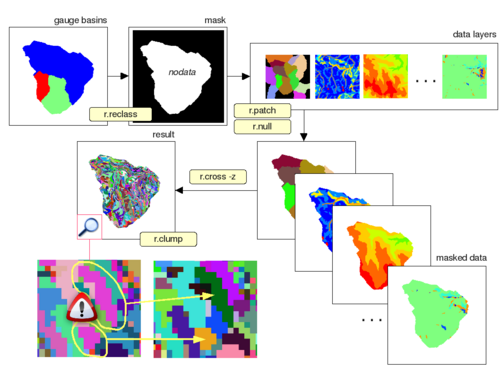
\includegraphics[width=\textwidth]{layers}
      \caption[QGIS (in this example using the grass functionality) can be used to overlay different types of information;]
{QGIS (in this example using the grass functionality) can be used to overlay different types of information; source:~\url{http://geoinformatics.fsv.cvut.cz/gwiki/Deriving_Hydrological_Response_Units_\%28HRUs\%29_using_a_Web_Processing_Service_implementation_based_on_GRASS_GIS};}
      \label{layers} % so that one can \ref it elsewhere	
    \end{center} 
  \end{figure}

Bellow are examples of some specific (and common) problems with catch data, for which we propose to develop some solutions in the system.% One is that we are missing data from our sampling universe (for instance it is an outlier or simply it was not sampled); the other is the data exists, but it is incomplete since the 

\begin{itemize}
  \item \textbf{Imputation of missing data}: Under-sampled or non sampled strata lead to an unknown bias, a problem that should be reduced with a good sampling design~\cite{ices}. For the situations where we have to deal with missing values, it is possible to inmputate them, having in mind that also the method used for this operation can introduce some bias in the system. According to ICES~\cite{ices} automatic methods should be avoid, in favor of expert knowledge, but they can be aided by spatial modelling techniques having in mind that to be use with success the spatial distribution should remain stable over time; this is a cue for developing GIS based models, that can provide the expert with a good basis for informed choices.

  \item \textbf{Allocate Catch in undefined areas}: On the Canadian Albacore Tuna Catch and Effort Relational Database~\cite{tuna} it is presented the problem of having sales or logbook catch data, whose geographic area is undefined. Instead of discarding these values from the calculations of catch by area, the authors found ways to distribute the catch and effort, following the overall geographic pattern of fleet; they allocate these values in proportion with the total catch and vessel distribution and for this purpose GIS can be very useful, for instance to produce a grid, or a contour map (see figure~\ref{kernel}) with frequencies.

  \item \textbf{Estimate known unreported catch}: Another delicate problem arises from the incomplete vessel count. If there is an unreported effort than it will probably be reflected in an unreported catch. For the cases where it is known that an unreported effort exists, the authors of the the Canadian Albacore Tuna Catch and Effort Relational Database~\cite{tuna} suggest to extrapolate the total catch estimates based, on estimated number of unreported vessels. According to~\cite{morocco}, unreported catch can be as significant as 50\% of the total catch and therefore it is important to find suitable methods to approach this problem, like for instance the Monte Carlo Simulation (see figure~\ref{montecarlo}).

\end{itemize}

  \begin{figure}[!ht]%[htbp]
    \begin{center} 
	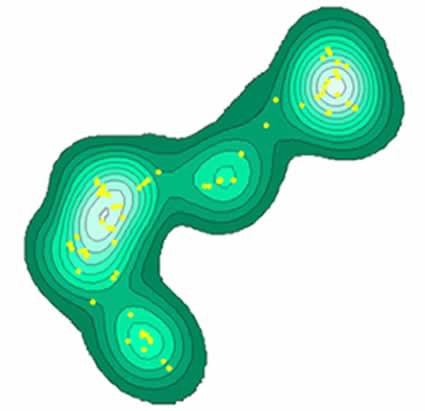
\includegraphics[width=0.5\textwidth]{kernel}
      \caption[The Kernel Home Range Method is a probability measurement that outputs contours, based on ponctual observations;]
{The Kernel Home Range Method is a probability measurement that outputs contours, based on ponctual observations; source:~\url{http://www.bio.davidson.edu/people/midorcas/GISclass/GISprojects/grayson/GISMethods.htm};}
      \label{kernel} % so that one can \ref it elsewhere	
    \end{center} 
  \end{figure}

  \begin{figure}[!ht]%[htbp]
    \begin{center} 
	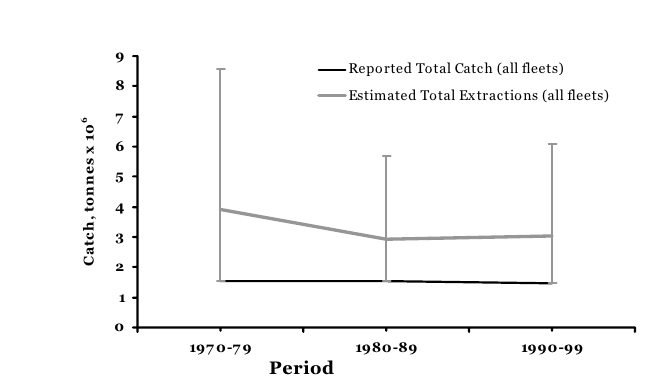
\includegraphics[width=\textwidth]{montecarlo}
      \caption[In this example, Monte Carlo Simulation was used to elaborate estimates of total extractions of all species from Moroccan waters; in the image we see the comparison with the total reported catch;]
{In this example~\cite{morocco}, Monte Carlo Simulation was used to elaborate estimates of total extractions of all species from Moroccan waters; in the image we see the comparison with the total reported catch;}
      \label{montecarlo} % so that one can \ref it elsewhere	
    \end{center} 
  \end{figure}

%Apart from this, interpolation/extrapolation algorithms could be developed to deal with different types of information (effort, catch, climatological data, etc).

\subsection{Data Output}\label{output}
Data output, of raw or transformed information, is a component where it is possible (and desirable) to facilitate the link with other platforms by using "friendly" and well-known formats. This could include formats for tabular data (for excel, R, etc), but also formats for spatial data (shapefiles, GeoJSON,etc).\\
GIS provide some very-rich and expressive visualization tools with a great potential for fisheries data, that we will discuss summarily in the next few paragraphs.\\
Web mapping is the process of designing, implementing, generating and delivering maps on the World Wide Web~\footnote{\url{http://en.wikipedia.org/wiki/Web_mapping}}. Compared to "traditional" maps, maps on the Internet have many other advantages such as "live updating", and link with many other sources of information; they provide the same interactivity as a GIS software, with the advantage of not requiring a specific software client, since they can run on an Internet browser. Web maps are normally incorporated in portals, together with other types of information, like in the case of ICES Ecosystem Data~\cite{ices2} (see figure~\ref{webmap}), but they can also be embedded in a software application (see figure~\ref{marble}).

  \begin{figure}[!ht]%[htbp]
    \begin{center} 
	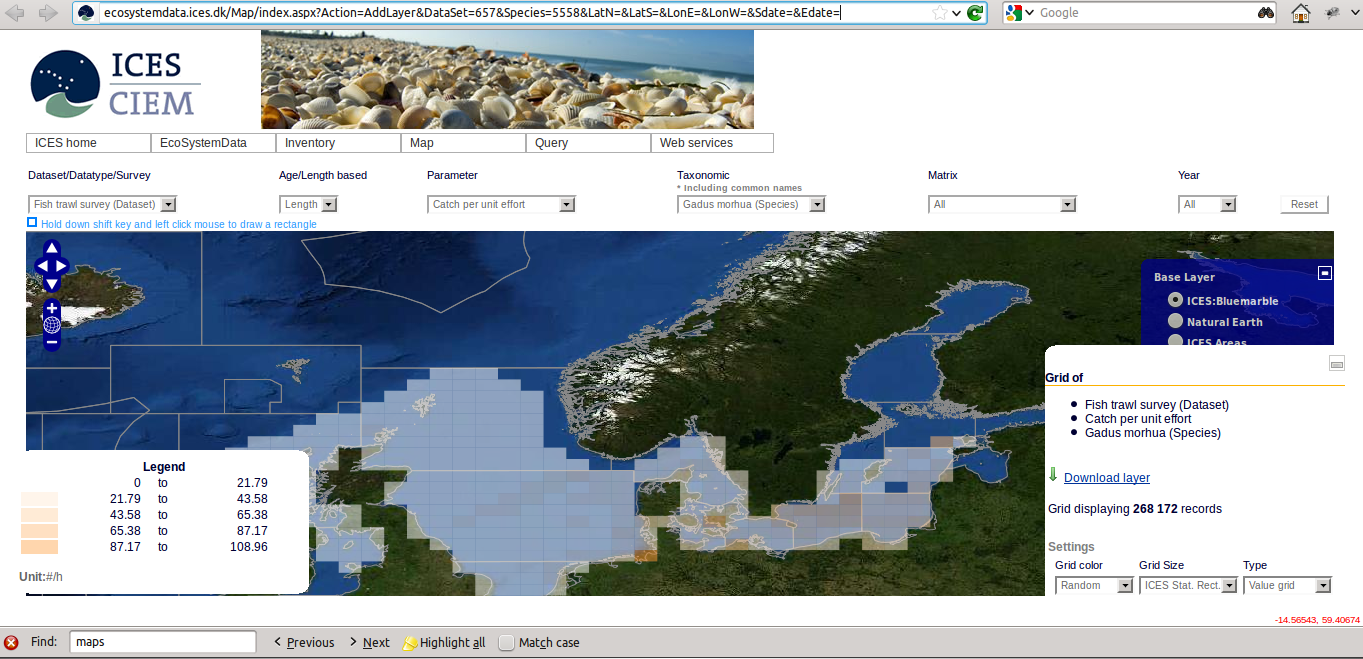
\includegraphics[width=\textwidth]{webmap}
      \caption[Web map of a ICES fish trawl Survey dataset, overlaying a grid of CPUE on top of a layer of Marble (Nasa Worldwind);]
{Web map of a ICES fish trawl Survey dataset, overlaying a grid of CPUE on top of a layer of Marble (Nasa Worldwind)~\cite{ices2};}
      \label{webmap} % so that one can \ref it elsewhere	
    \end{center} 
  \end{figure}

  \begin{figure}[!ht]%[htbp]
    \begin{center} 
	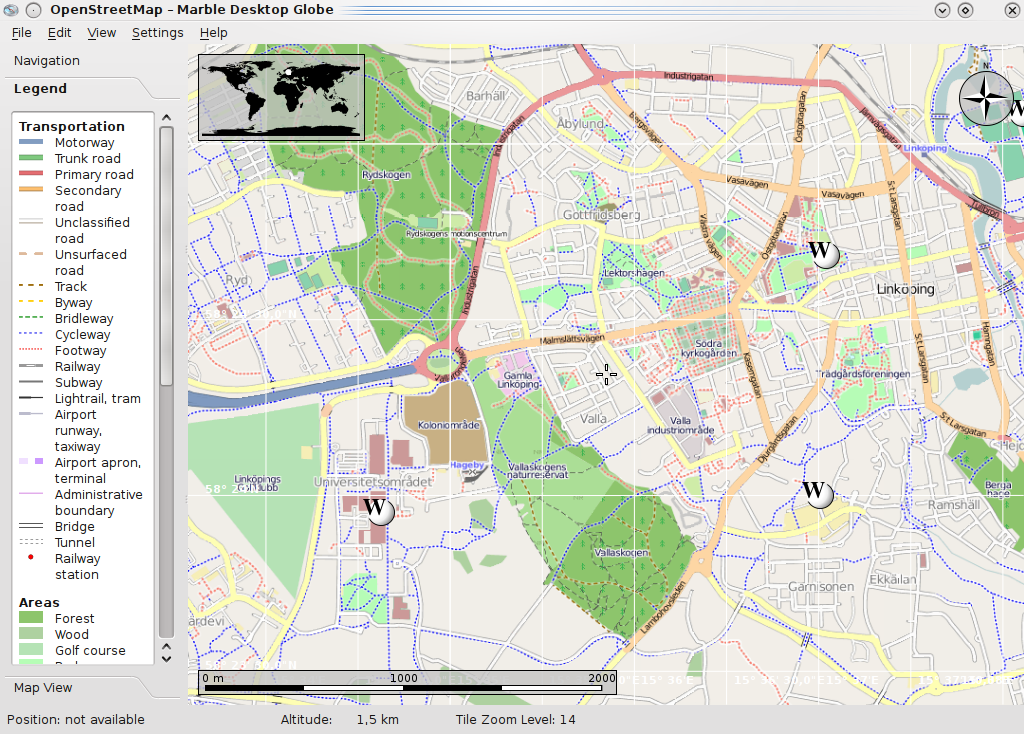
\includegraphics[width=\textwidth]{marble}
      \caption[Marble is a free and open source application that displays webmaps, along with other types of maps in a C++ application;]
{Marble~\footnote{\url{http://edu.kde.org/marble/}} is a free and open source application that displays webmaps, along with other types of maps in a C++ application; source:~\url{http://edu.kde.org/marble/screenshots/generic/marble-linkoeping.png};}
      \label{marble} % so that one can \ref it elsewhere	
    \end{center} 
  \end{figure}

Continuous maps showing densities, can be created using grids or contours or other methods such as TINs. Grids (such as the one on figure~\ref{webmap}) are very common to represent distributions of fishing effort or catches; On the Geocrust project (see~\cite{geocrust}), the generation of grids with different sizes allowed the user to have a more generalized or more detailed perception of the fishing effort, which calls its attention to different properties (see figure~\ref{grids}).

\begin{figure}[ht]
\centering
\subfigure[Density map of fishing effort, using a large grid;]{
   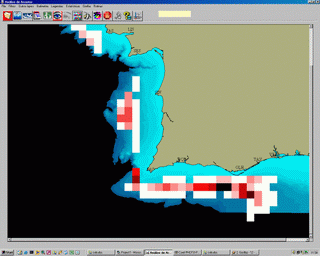
\includegraphics[width=0.8\textwidth] {densidades99_5x5}
 }
 \subfigure[Density map of fishing effort, using a small grid;]{
   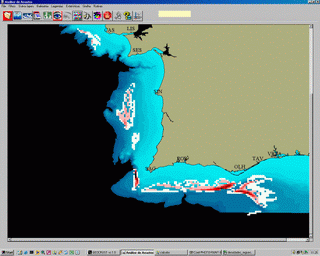
\includegraphics[width=0.8\textwidth] {densidades99a.png}
 }
\caption[Fishing effort maps generated by GeoCrust 2.0. To produce these maps the user can choose one or more vessels for a given period of time quarter, semester, and year); VMS data from valid fishing trips trawl hauls. Density grid size set by the user (minimum 0.06 x 0.06 nm);]
{Fishing effort maps generated by GeoCrust 2.0. To produce these maps the user can choose one or more vessels for a given period of time (quarter, semester, and year); VMS data from valid fishing trips trawl hauls. Density grid size set by the user (minimum 0.06 x 0.06 nm);}
\label{grids}
\end{figure}

GIS functions for cartography are generally based on boolean logic: that is, sharp frontiers between entities. However, when there is uncertainty and vagueness attached to a certain phenomena, this "false" precision may be awkward or simply inadequate (see~\cite{fuzzy2}). The Zadeh’s fuzzy set theory is an alternative to this boolean logic and has been proposed has a foundation to GIS design, that can be incorporated to cartographic display of phenomena with a certain imprecision associated to them. On figure~\ref{fuzzy} we see the comparison of a traditional map, with sharp boundaries and a fuzzy map.\\
On fisheries surveys, where often spatial data relies on human description (for instance a fishermen describing where he was fishing), this could provide a very interesting approach.

  \begin{figure}[!ht]%[htbp]
    \begin{center} 
	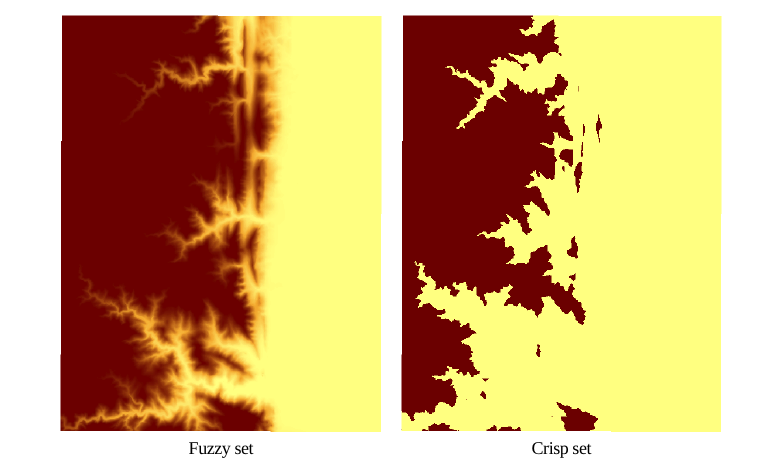
\includegraphics[width=\textwidth]{fuzzy}
      \caption[This is an illustrative example of an analysis with a fuzzy logic approach (left) and a crisp approach (right);]
{This is an illustrative example of an analysis with a fuzzy logic approach (on the left) and a crisp approach (on the right)~\cite{fuzzy3};}
      \label{fuzzy} % so that one can \ref it elsewhere	
    \end{center} 
  \end{figure}

%A cutting-edge area of computation that has a great potential for fisheries applications is fuzzy mapping. A Fuzzy cognitive map is a map within which the relations between the elements (e.g. concepts, events, etc) of a "mental landscape" can be used to compute the "strength of impact" of these elements~\footnote{\url{http://en.wikipedia.org/wiki/Fuzzy_cognitive_map}}.

%speak about GEOCRUST (maps) and fuzzy maps, ICES (Web mapping)
%link to other platforms
% open source, agile


%\section{Project Outputs}\label{outputs}
%Write something here

%\section{Work Plan}\label{plan}
%Write something here

%\section{Capacity Building Components}\label{capacity}
%Write something here

%\section{FAO Input}\label{fao}
%Write something here

%\section{Recipient Countries Input}\label{countries}
%Write something here

%\section{Project Budget}\label{budget}
%Write something here

%AKNOWELEDGMENTS

%\section{Project Outputs}\label{outputs}
%Write something here

\section{Aknoweledgments}
I would like to thank Henrik Degel, from the Fishframe project, for kindly providing me with a login that allowed me to try the Fishframe system; Carlos Pinto, from ICES, for amending and "filling the gaps" for the ICES systems reviewed on section~\ref{context}; and Fabio Carocci, from FAO, for suggesting me to review a prorietary GIS fishery system.

\clearpage

\begin{thebibliography}{9}
\bibitem{fishframe}F.\ Degel, T.\ Jansen {\em FishFrame Fisheries and stock assessment data framework}. ICES CM 2006/M:02
, 2006.
\bibitem{fishframe1}F.\ Degel, T.\ Jansen {\em FishFrame Licensing}.Danish Institute for Fisheries Research
Charlottenlund castle, Charlottenlund, Denmark. 5th March, 2006.
\bibitem{intercatch}H.\ Kjems-Nielsen, L. \ Inger Larsen, M.\ Zarecki1, T.\ Jansen, B.\ Cowan, P.\
Sandbeck, M.\ Dueholm, O.\ Skov.{\em InterCatch - a tool for fish stock assessment, status and methods}. ICES CM 2006/M:29, 2006.
\bibitem{intercatch1}ICES. {\em InterCatch - User Manual.}. Document version 1.9.
\bibitem{EcoSystemData}ICES {\em EcoSystemData3.0\_Release}. \url{http://ecosystemdata.ices.dk/EcoSystemData3.0_Release.pdf}
\bibitem{tuna}M.\ Stocker, H.\ Stiff, W.\ Shaw, A.W.\ Argue {\em The Canadian Albacore Tuna Catch and
Effort Relational Database}. Canadian Technical Report of Fisheries and Aquatic Sciences 2701, 2007.
\bibitem{mappamond}Mappamond {\em Fishery\_Analyst\_V2\_manual}. \url{http://www.mappamondogis.it/pdf/Fishery_Analyst_V2_manual.pdf}
\bibitem{victoria}L.I.\ Muhoozi {\em Implementation of a Fisheries Management Plan
(IFMP) Project for Lake Victoria: A Report Of The Fisheries Catch Assessment Survey
In The Ugandan Waters Of Lake Victoria For The February 2008 Survey}. National Fisheries Resources Research
Institute (NaFIRRI) and National Agricultural Research
Organization (NARO), February, 2008.
\bibitem{dominican}P. A.\ Medley {\em Review Of The Data Collection And Management
Systems Of The Marine Fisheries In The Dominican
Republican: Final Report}.
\bibitem{samoa}N.\ Helm {\em A Report on The Market Survey of Reef and Lagoon Fish Catches In Western
Samoa}. South Pacific Comission, SPC/lnshoreFish.Res./BP 30, 7 March 1988.
\bibitem{medfisis} FAO.\emph{Medfisis},\url{http://www.faomedfisis.org/}.
\bibitem{json} JSON.\emph{JSON},\url{http://json.org/}.
\bibitem{sqlite} SQLite.\emph{SQlite},\url{http://www.sqlite.org/}.
\bibitem{fuzzy}H.H.\ Shahri, A.A.Z.\ Barforush.{\em Data mining for removing fuzzy duplicates using fuzzy inference}.
Fuzzy Information, 2004. Processing NAFIPS '04. IEEE Annual Meeting, 27-30 June 2004. \url{http://ieeexplore.ieee.org/xpl/freeabs_all.jsp?arnumber=1336319}
\bibitem{outliers}C.\ López.{\em Quality of Geographic Data
Detection of Outliers and Imputation of
Missing Values}. PhD Dissertation on the Royal Institute of Technology, Department of Geodesy and Photogrammetry, Stockholm, Sweden 1997.
\bibitem{ices}ICES.{\em Workshop on methods for merging metiers for
fishery based sampling (WKMERGE)
}. ICES WKMERGE REPORT 2010, Copenhagen, Denmark, 19-22 January 2010.
\bibitem{morocco}R.\ Forrest, T.\ Pitcher,
R.\ Watson, H.\ Valtýsson,
S.\ Guénette {\em Estimating Illegal and Unreported Catches from Marine Ecosystems: Two Case Studies}. Sea Around Us: North Atlantic, Page 81, 19 DEC 2002.
\bibitem{ices2} ICES.\emph{ICES Data Centre},\url{http://www.ices.dk/datacentre/Submissions/index.aspx}.
\bibitem{geocrust}J.\ Simoes, C.\ Pinto, M.\ Afonso-Dias. {\em Methodology for Monitoring and  Management of the Crustacean Trawl Fleet. Example of GeoCrust 1.0 GIS} in Finisterra special edition Cartography and Geographic Information Systems, 2005.
\bibitem{fuzzy2}D. Z.\ Sui {\em A Fuzzy Gis Modeling Approach Land Evaluation For Urban}. Environ. and Urban Systems, Vol. 16, pp. IOl-115, USA, 1992.
\bibitem{fuzzy3}W.\ Kainz.{\em The mathematics of GIS}. \url{http://goo.gl/fb/CWklR}
\bibitem{fao1}FAO/DANIDA.{\em Guidelines for the Routine Collection of Capture Fishery Data}. FAO FISHERIES TECHNICAL PAPER 382. Food and Agriculture Organization of the United Nations. Rome, 1999.
\bibitem{bd}{\em fisheries\_data\_mng\_sys.sqlite}.
\bibitem{first}L. R.\ Garces, G. T.\ Silvestre, I.\ Stobutzki, F. C.\ Gayanilo Jr, F.\ Valdez, M.\ Saupi, T.\ Boonvanich, M.\ Roongratri, P.\ Thouc, Purwanto, I.\ Haroon, K. N.\ Kurup, M.\ Srinath, H. A. B.\ Rodrigo, M. D.\ Santos, F. S. B. Torres Jr., M. K.\ Tan, D.\ Pauly {\em A regional database management system—the fisheries resource information system and tools (FiRST): Its design, utility and future directions}. Fisheries Research, 78 (1-2). pp. 119-129.
\bibitem{pescart}IIP.{\em PESCART: Documentacao tecnica}. 2006.
\bibitem{cost}European Comission.{\em Common tool for raising and estimating properties of statistical estimates derived from the Data Collection Regulation (COST)}. Studies and Pilot projects for carrying out the common fisheries policy. Call for proposal FISH/2006/15 – lot 2.
\bibitem{cost1}COST Team and various contributors.{\em Package ‘COSTcore’ documentation}. February, 15, 2008.
\bibitem{kongatora}B. U.\ Ibrahim, J.\ Auta, J. K.\ Balogun,{\em A Survey Of The Artisanal Fisheries Of Kontagora Reservoir, Niger State, Nigeria}. Bayero Journal of Pure and Applied Sciences, 2(1): 47 - 51. 2009.

\end{thebibliography}



\end{document}